\documentclass{article}
\usepackage[a4paper, total={6in, 9in}]{geometry}
\usepackage{wrapfig}
\usepackage{booktabs}
\usepackage{graphicx}
\usepackage{float}
\title{Allowances and Universal Basic Income}
\author{Nikhil Woodruff}

\begin{document}
    \maketitle
    \section{Introduction}
    Allowances are sections of the tax-benefit system which disregard income for the purposes of tax and benefit calculations. They often provide significant tax reliefs and 
    \section{Personal Allowance}
    The Personal Allowance is an allowance for most UK individuals, deductible from all forms of income for Income Tax. It is the largest and fastest-growing allowance in the tax code, with most of its gains seen during the Coalition government of 2010-2015, currently standing at £12,570 per year. Figure \ref{fig:PA_hist} shows historical levels of Income Tax allowances, in context with the Personal Allowance: only the Blind Person's Allowance has remained such a consistent component of the tax system.
    \begin{wrapfigure}{i}{0.6\textwidth}
        \centering
        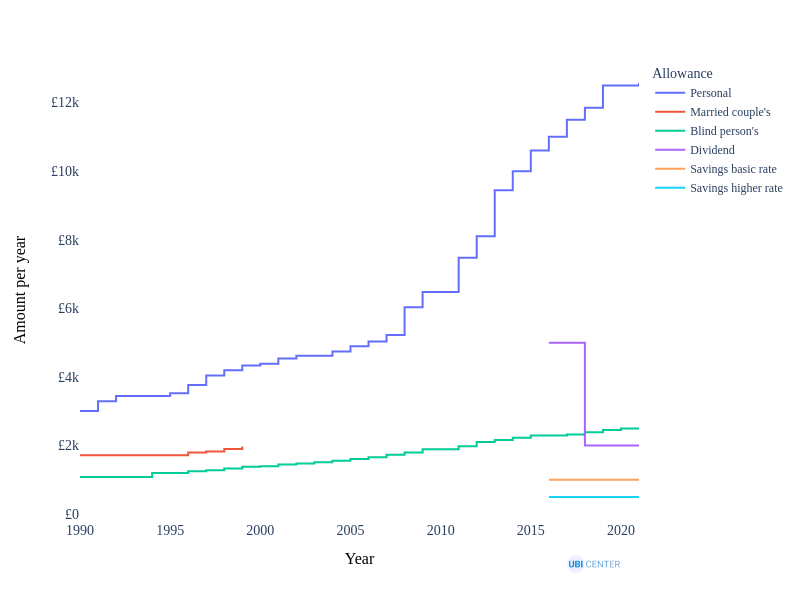
\includegraphics[width=0.6\textwidth]{images/fig_1.png}
        \caption{Historical allowance levels}
        \label{fig:PA_hist}
    \end{wrapfigure}

    \subsection{Current System}

    \paragraph{Effects on income}

    From its effect on taxable income, the Personal Allowance significantly decreases Income Tax revenue. Using the OpenFisca-UK microsimulation model, I estimate that the reduction in Income Tax revenue caused by the allowance was approximately £105.9bn in 2020. 
    
    However, this does not equal the net revenue raised by its abolition - the Personal Allowance, by increasing post-tax income, reduces necessary welfare spending. For example, for each £1 increase in post-tax income for an individual on the Universal Credit taper, the benefit amount is decreased by 63p. 
    
    Conversely, decreasing the individual's post-tax income by reducing the Personal Allowance would necessitate increases in total government spending on means-tested welfare benefits. I estimate that, after taking increases in benefit spending into account, the total revenue raised by the abolition of the Personal Allowance per year would be £98.3bn.
    
    \paragraph{Margin effects} Figure \ref{fig:PA_mtr_effects} shows the changing effective marginal tax rate (the percentage of an extra £1 of income which would not income an individual's disposable income after taxes and benefits) over the income spectrum for a hypothetical individual\footnote{For this example, we assume the individual claims all benefits to which they are eligible and pays all taxes for which they are liable.}. 
    
    The Personal Allowance is applicable to the vast majority of UK individuals, but some are excluded by the use of means-testing: individuals with an adjusted net income (taxable income) of over £100,000 begin to see their Personal Allowance phased out at a rate of 50\% as they increase taxable income. This increases tax revenue, but creates a period of higher marginal tax rates for earnings in the region, reaching an effective marginal tax rate of 60\% for the income range between £100,000 and £125,000.

    \begin{wrapfigure}{O}{0.6\textwidth}
        \centering
        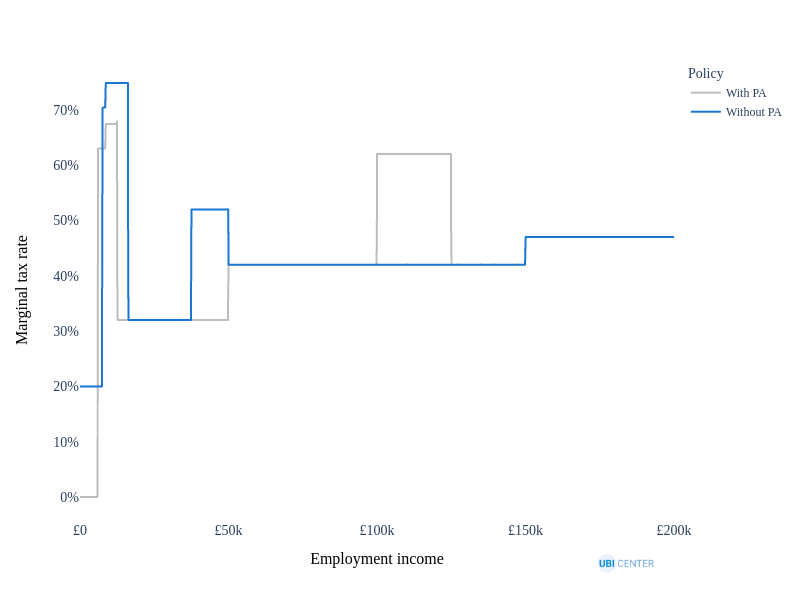
\includegraphics[width=0.6\textwidth]{images/fig_2.png}
        \caption{Marginal tax rate effects of the Personal Allowance}
        \label{fig:PA_mtr_effects}
    \end{wrapfigure}
    
    The Personal Allowance also reduces marginal tax rates at the lower end of the income spectrum, but the effect is smaller than 20\% as reductions in tax MTRs are partially offset by increases in benefit phaseout. The allowance shortens the region of punitively high effective marginal tax rates caused by benefit withdrawal by this effect, and its synchronisation with the National Insurance Upper Earnings Limit avoids a sharp increase in marginal tax rates shortly for middle-income earners.

    \begin{wrapfigure}{I}{0.6\textwidth}
        \centering
        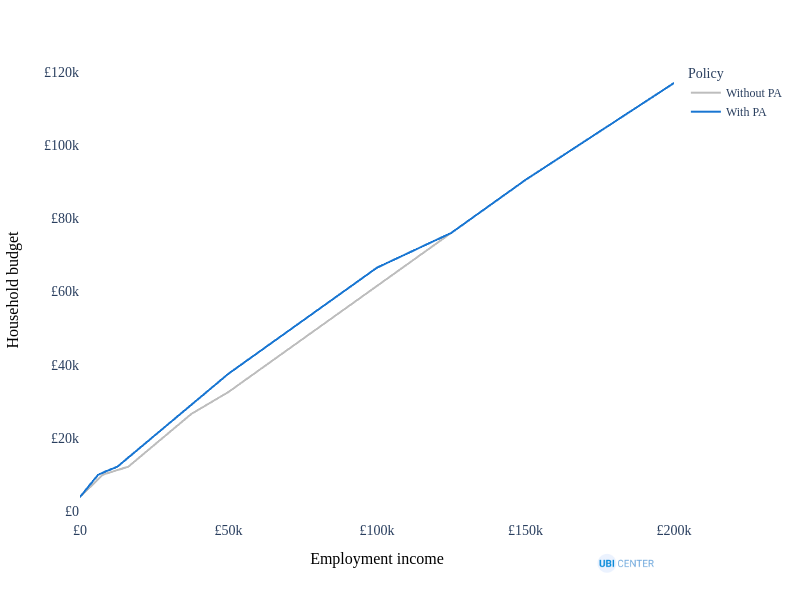
\includegraphics[width=0.6\textwidth]{images/fig_3.png}
        \caption{Budget effects of the Personal Allowance}
        \label{fig:PA_budget_effects}
    \end{wrapfigure}

    \paragraph{Budget effects} The gain seen by individuals is maximised in the higher income regions, between £50,000 and £100,000. However, its inclusion in the tax code is disproportionately beneficial in absolute amount to those on higher incomes before the phase-out (due to the fact that it effectively delays the current marginal tax rate schedule, which increases monotonically within the range of the Personal Allowance). As shown by Figure \ref{fig:PA_budget_effects}, absolute financial gain increases with income (before the phase-out).

    \subsection{UBI Replacement}

    Repealing the Personal Allowance raises a significant amount of increased tax revenue, posing the question of how the socio-economic effects of this revenue might differ if distributed as a universal basic income, rather than a tax cut. The details of such a UBI policy are simple: each adult and child citizen of the United Kingdom receives an equal payment: a share of the total available funds (maintaining budget neutrality). UBI payments are not included as income in means-tested benefits, allowing those on low incomes to receive the full benefit of the payment. The static results of such a reform are given in Table \ref{tab:PA_UBI_results}.
    \begin{table}
        \centering
        \begin{tabular}{llll}
            \toprule
            Category & Metric & Absolute & Relative \\
            \midrule
            Distributional & Median income (£k) &        1.0 &      2.7 \\
                    & Gini coefficient &     -1.6 &     -4.1 \\
            Poverty & Overall rate (pp) &     -4.2 &    -31.1 \\
                    & Deep poverty rate (pp) &     -1.1 &    -45.5 \\
                    & Adult poverty rate (pp) &     -3.3 &    -30.2 \\
                    & Senior poverty rate (pp) &     -0.1 &     -0.5 \\
                    & Child poverty rate (pp) &    -10.4 &    -53.7 \\
                    & Poverty gap (£bn) &     -7.2 &    -36.1 \\
            Fiscal & Tax revenue (£bn) &    105.9 &     46.8 \\
                    & Benefit spending (£bn) &    106.4&       56 \\
            Overall & Winners &     52.2 &        - \\
                    & Losers &     47.6 &        - \\
            \bottomrule
        \end{tabular}
        \caption{Static effects of a PA-UBI exchange}
        \label{tab:PA_UBI_results}
    \end{table}
    
    In order to provide comparability for the reforms in this paper, results are categorised in to distributional (inequality and median income), poverty (rates for specific groups and the poverty gap), fiscal (budgetary effects) and overall (percentage net winners and losers). 
    
    \paragraph{Distributional} The Gini coefficient is a measure of inequality ranging between 0 (complete equality) and 1 (maximal inequality, with all income concentrated on one entity). In these results, the Gini coefficient is calculated over the equivalised (adjusted for household composition) household disposable income for every person (adult and child) in the population. It is to be expected that this reform reduces the Gini coefficient in static terms, as raising tax rates and flat amount spending is inherently progressive.
    
    \paragraph{Poverty} These results show significant reductions in poverty rates among all major demographic groups, with the strongest effects seen on child poverty. Child poverty levels are generally reduced more than others by universal basic income reforms that include children and are funded by taxation, as households with children have a lower per-capita tax liability (children mostly having no taxable income). 
    
    Figure \ref{fig:poverty_rates_hist} shows the trend of poverty rates over the last two decades for context. While trends are decreasing for absolute indicators, this is gradual not always consistent; an exchange of the Personal Allowance for a UBI would outperform the absolute, before housing costs poverty rate reduction for every year in recent history.

    \begin{wrapfigure}{O}{0.6\textwidth}
        \centering
        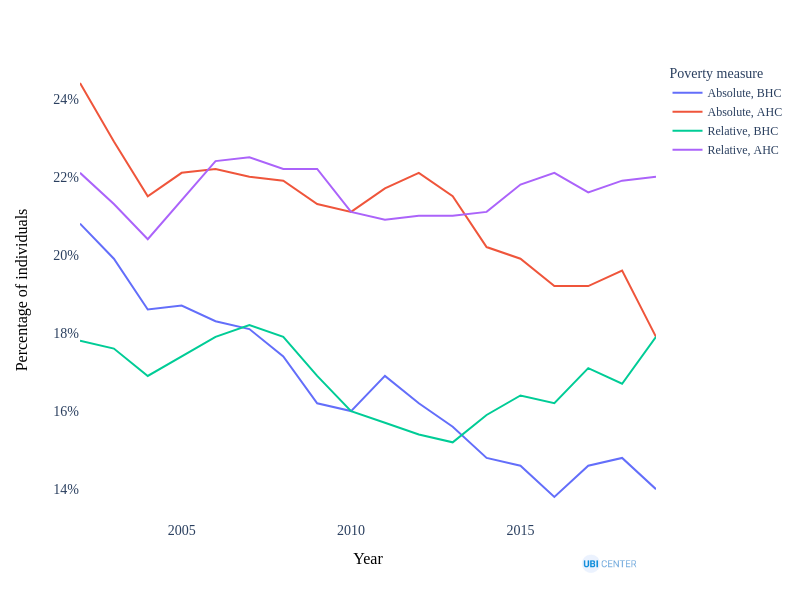
\includegraphics[width=0.6\textwidth]{images/fig_5.png}
        \caption{Historical poverty rates}
        \label{fig:poverty_rates_hist}
    \end{wrapfigure}
    
    Deep poverty is defined as living in a households whose disposable income is less than half of the poverty line. The poverty gap is the sum of the positive shortfalls between households' disposable incomes and their poverty lines - the minimum total funds required to eliminate poverty. This is a more informative measure of the poverty situation of the country, since the poverty rate does not treat separately households just below the poverty line, and those in deep poverty. This reform reduces deep poverty by just over 45\% and the poverty gap by 36\%, a significant reduction.

    \section{Primary Threshold and Lower Profits Limit}

    The National Insurance Primary Threshold and Lower Profits Limit are a tax elements which remove sections of employment and self-employment income, respectively, from the tax base. Their abolition would raise taxes on earned income, and are an alternative or complementary funding method for universal basic income than abolishing the Personal Allowance.

    \subsection{Current System}
    National Insurance, separate to Income Tax, is a tax on employment and self-employment income for individuals under State Pension Age. It consists of four separate classes: Class 1, on employment income for both employees and employers; Class 2, a flat rate on self-employment income; Class 3, voluntary contributions to maintain access to associated benefits; and Class 4, a marginal rate on self-employment income.

    Defined within Class 1 are Primary (employee-side) and Secondary (employer-side) contributions, in addition to Class 1A and 1B rates, paid by employers on expenses and benefits paid to employees. Thresholds are technically distinct from allowances - reducing an allowance lowers thresholds above it, whereas reducing thresholds do not affect higher thresholds. We still consider the abolition of the lowest NI thresholds in this paper due to their similarity as a tax base-widening mechanism. 

    \begin{wrapfigure}{I}{0.6\textwidth}
        \centering
        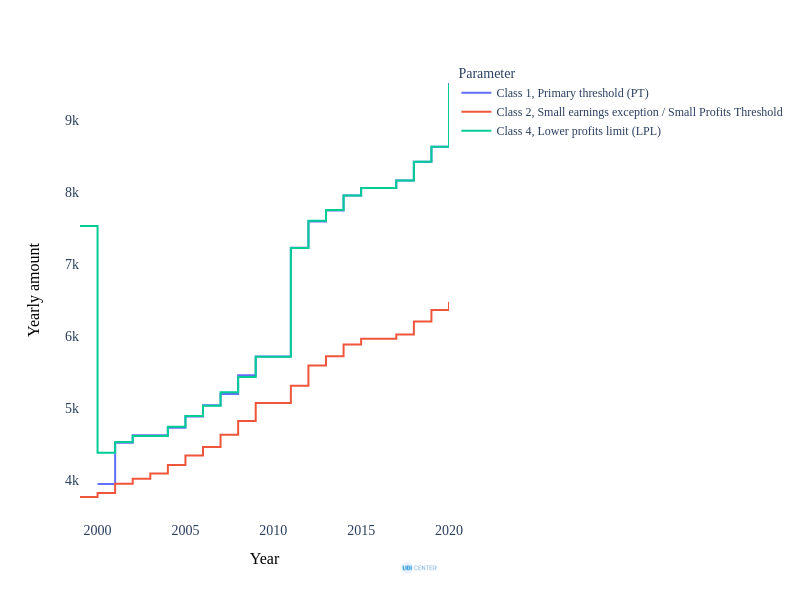
\includegraphics[width=0.6\textwidth]{images/fig_6.png}
        \caption{Historical NI thresholds}
        \label{fig:NI_thresholds}
    \end{wrapfigure}

    Shown in Figures \ref{fig:NI_thresholds} and \ref{fig:NI_rates}, thresholds and rates have broadly risen over time. The fastest rise in thresholds took place during 2011, when the Primary Threshold and Lower Profits Limit were raised by over £1,000 per year. Rises since then have been consistent, with an increase for 2021.
    
    \begin{wrapfigure}{O}{0.6\textwidth}
        \centering
        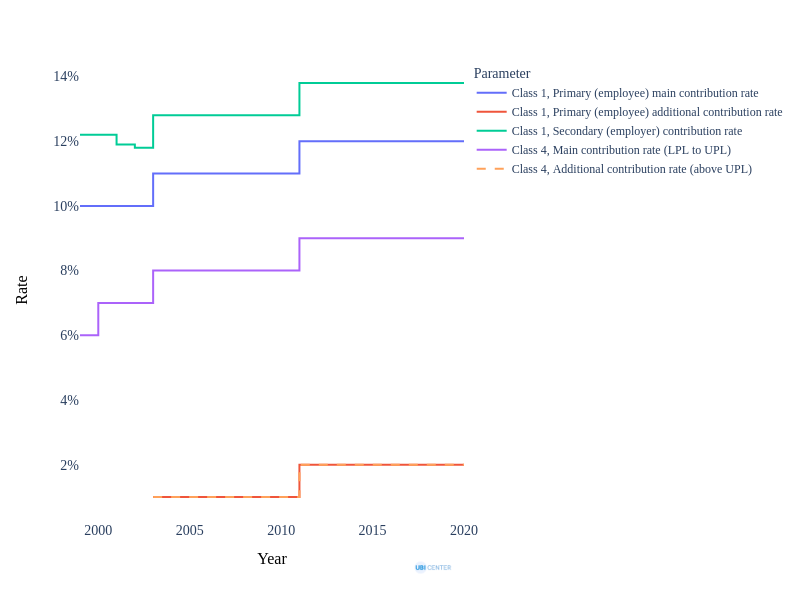
\includegraphics[width=0.6\textwidth]{images/fig_7.png}
        \caption{Historical NI rates}
        \label{fig:NI_rates}
    \end{wrapfigure}

    Rates have largely remained consistent since 2003, with a one-point rise in all rates by the Labour governments during 2003 and 2011, to fund increased health expenditure.

    \paragraph{Self-employment} The current system provides a lower tax burden for the self-employed - NI (and total tax) contributions are lower at most points in the income spectrum, except for a region caused by the flat rate of Class 2 contributions. The main cause of the difference between employed and self-employed earnings taxation is caused by the reduced main rate of 9\% for the self-employed, compared to 12\% for employees. 
    
    This also makes no assumption about how employer contributions affect employee pay, which would widen the gap further between employment and self-employment tax treatment. Since this paper only considers allowance and threshold reductions to fund UBI expenditure, this treatment difference, which can only be removed by equalising the main rates of National Insurance, is unchanged by the UBI reform.

    \begin{wrapfigure}{I}{0.6\textwidth}
        \centering
        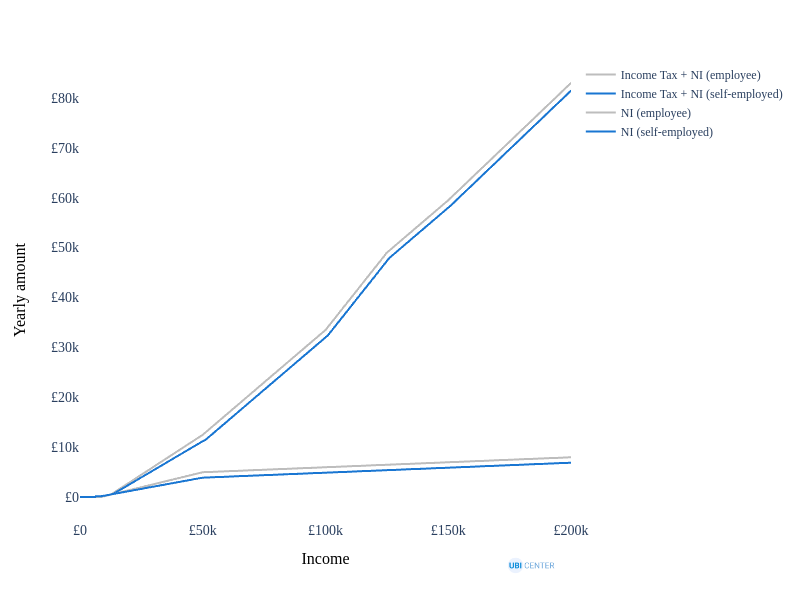
\includegraphics[width=0.6\textwidth]{images/fig_8.png}
        \caption{NI contributions for the employed and self-employed}
        \label{fig:NI_self_emp_diff}
    \end{wrapfigure}

    \paragraph{Margin effects} The PT/LPL tax reliefs do not change effective marginal tax rates as strongly as the Personal Allowance, due to the fact that National Insurance imposes much lower tax rates than Income Tax. There are, however, some changes for low-income earners, shown in Figure \ref{fig:NI_mtr_effects}: the allowance eliminates effective MTRs at earnings close to zero and transitions individuals off means-tested benefits earlier than without the allowance, due individuals' applicable income for benefit programs being higher with the tax cut caused by the Primary Threshold and Lower Earnings Limit.

    \paragraph{Benefit considerations} Unlike Income Tax, National Insurance payment histories affect the payment of benefits such as the State Pension, contribution-based Jobseeker's Allowance or contribution-based Employment and Support Allowance. These programs require individuals to have a record of National Insurance payments, using specific, lower thresholds such as the Lower Earnings Limit (£120/week in 2021): individuals who earn above this threshold qualify for the benefits tied to National Insurance history. Tax reforms that remove these requirements of align the differences between employees and self-employed individuals in their entitlement based on payments are out of the scope of this paper, and therefore no change to this system is modeled.

    \begin{wrapfigure}{O}{0.6\textwidth}
        \centering
        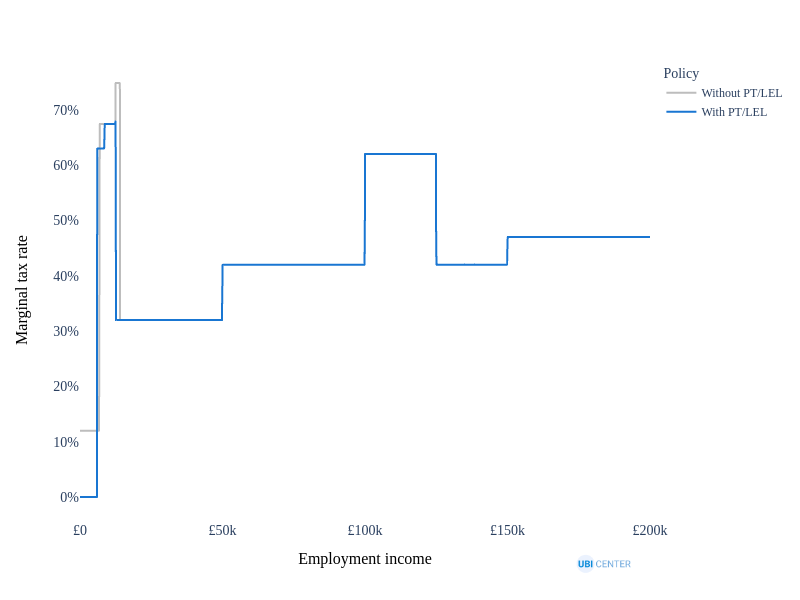
\includegraphics[width=0.6\textwidth]{images/fig_9.png}
        \caption{Effective marginal tax rate changes from the NI allowances}
        \label{fig:NI_mtr_effects}
    \end{wrapfigure}

    \subsection{UBI Replacement}

    \begin{table}
        \centering
        \begin{tabular}{llll}
            \toprule
            Category & Metric & Absolute & Relative \\
            \midrule
            Distributional & Median income (£k) &       -0 &       -0 \\
                    & Gini coefficient &     -0.6 &     -1.5 \\
            Poverty & Overall rate (pp) &     -1.4 &    -10.4 \\
                    & Deep poverty rate (pp) &     -0.5 &    -19.6 \\
                    & Adult poverty rate (pp) &     -0.8 &     -7.5 \\
                    & Senior poverty rate (pp) &       -2 &    -12.3 \\
                    & Child poverty rate (pp) &     -2.7 &    -14.1 \\
                    & Poverty gap (£bn) &     -2.7 &    -13.3 \\
            Fiscal & Tax revenue (£bn) &     29.1 &     12.9 \\
                    & Benefit spending (£bn) &     29.3 &     15.4 \\
            Overall & Winners &     53.4 &        - \\
                    & Losers &     46.3 &        - \\
            \bottomrule
        \end{tabular}
        \caption{Static effects of exchanging the PT and LPL for a UBI}
        \label{tab:NI_UBI_effects}
    \end{table}

    The removal of zero-rated parts of National Insurance would entail setting the Primary Threshold and the Lower Profits Limt to zero. Lowering the Small Earnings Exception, above which a flat rate of £3.05 per week is mandated, is therefore not necessary. This reform generates static estimated effects shown in Table \ref{tab:NI_UBI_effects}.

    \paragraph{Distributional} Changes to National Insurance affect fewer people (only employees and the self-employed under State Pension Age), and for those that are affected, financial effects are smaller than the repeal of the Personal Allowance. Median income does not significantly change, and the reduction in the Gini coefficient is lower. 
    \paragraph{Poverty} Poverty effects are smaller than the Personal Allowance-funded UBI overall and for children and working-age adults, but those over State Pension Age see a tangible reduction in the poverty rate, of around 12.3\%. This is expected, given that few senior citizens will be affected by the tax rises.\footnote{Few, but some are affected: while individuals of State Pension Age are not liable for National Insurance, their poverty status can still be altered if they live in a household close to the poverty line with any other person who is liable for NI.} Where repealing the Personal Allowance to fund a UBI provided only a very marginal 0.5\% reduction in senior poverty (due to the taxable status of the State Pension), the results here suggest that increases to NI contributions by widening the tax base can ameliorate some of the negative impact of Income Tax rises faced by pensioners.
    \paragraph{Fiscal} The revenue raised by the NI tax reforms is approximately one third as large as the repeal of the Personal Allowance, yet it still provides moderately strong antipoverty effects. This level of revenue is similar in nominal amount to main benefits such as Housing Benefit or Universal Credit.
    \paragraph{Overall} The percentage of individuals who come out ahead is slightly higher and the percentage who lose is slightly lower - reflecting a more concentrated burden on the working-age population and more distributed gains among the pensioner and child populations.

    \paragraph{Distributional comparison}

    \begin{wrapfigure}{I}{0.6\textwidth}
        \centering
        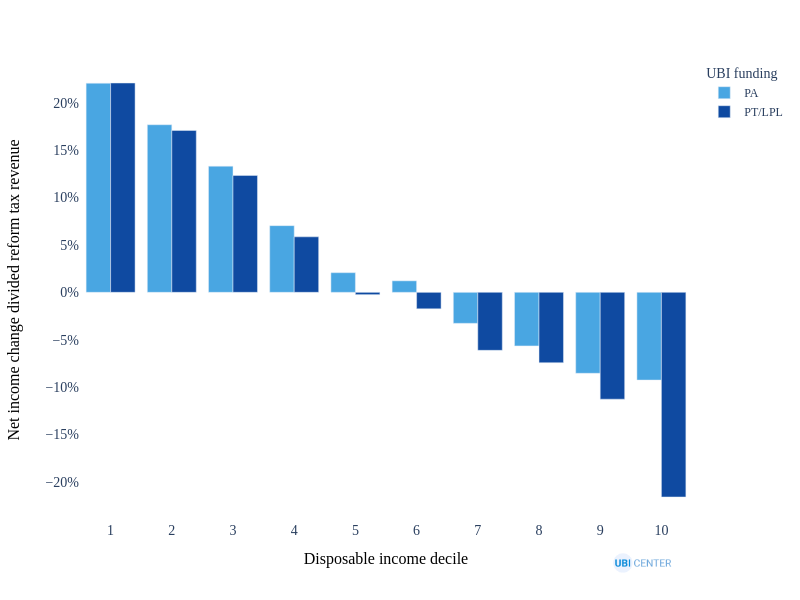
\includegraphics[width=0.6\textwidth]{images/fig_10.png}
        \caption{Share of the total UBI spending received by each decile}
        \label{fig:PA_NI_distr_comp}
    \end{wrapfigure}

    Both the Personal Allowance and the NI thresholds, exchanged for a UBI, produce progressive reforms. Figure \ref{fig:PA_NI_distr_comp} shows the share of total UBI spending received by the income deciles, making clear that while both are similar for most deciles, the National Insurance-funded UBI reform has a stronger relative impact on the top decile, due to the means testing of the Personal Allowance in the baseline system, limiting the impact of tax rises on individuals within that decile.

    \section{Smaller Allowances}

    While the Personal Allowance and the National Insurance thresholds are the largest potential sources of funds for a universal basic income, there are other elements of the tax-benefit system that could yield funding, and simplify the system in the process. These include the Dividend Allowance, Property Allowance, Trading Allowance, and Universal Credit Work Allowances. The Dividend Allowance allows individuals to disregard up to £2,000 of taxable income to reduce their tax liability. Previously at £5,000, it was reduced in 2017 (see Figure \ref{fig:PA_hist}). The Property Allowance applies to rental income of land or property, and currently stands at £1,000 per year. The Trading Allowance currently stands at £1,000 per year, and is deductible in place of deductions for expenses from self-employment or other trading income.

    The Universal Credit Work Allowance is an allowance for earned income which does not cause benefit reductions at the Universal Credit phase-out rate of 63\%. This varies by whether the family receives housing costs aid in their benefit payments. The current amounts are £293 with housing costs aid and £515 without. Table \ref{tab:small_UBI_results} shows the relative static effects of the exchange of each allowance with a UBI.

    \begin{table}[h]
        \centering
        \begin{tabular}{llllll}
            \toprule
            Category & Metric & Dividends & Property & Trading &  UC \\
            \midrule
            Distributional & Median income &      0.11 &     0.02 &   -0.03 &   0.32 \\
                    & Gini coefficient &     -0.07 &    -0.03 &   -0.03 &  -0.06 \\
            Poverty & Overall rate &     -0.23 &    -0.11 &    0.10 &   0.71 \\
                    & Deep poverty rate &     -0.30 &    -0.21 &    0.16 &  -0.67 \\
                    & Adult poverty rate &     -0.19 &    -0.16 &    0.20 &   2.73 \\
                    & Senior poverty rate &     -0.38 &    -0.10 &   -0.81 &  -2.03 \\
                    & Child poverty rate &     -0.20 &    -0.04 &    0.54 &  -0.75 \\
                    & Poverty gap &     -0.25 &    -0.20 &   -0.16 &  -0.39 \\
            Fiscal & Tax revenue &      0.45 &     0.15 &    0.26 &   0.00 \\
                    & Benefit spending &      0.53 &     0.18 &    0.31 &  -0.00 \\
            Overall & Winners &     79.30 &    95.00 &   88.90 &  90.80 \\
                    & Losers &     20.30 &     4.50 &   10.60 &   8.70 \\
            \bottomrule
        \end{tabular}
        \caption{Static (relative) effects of small allowance-UBI exchanges}
        \label{tab:small_UBI_results}
    \end{table}
    The estimated results from the abolition of small allowances are mixed, but poverty is reduced slightly by exchanging the Dividend and Property Allowances for a universal basic income, but increased by exchanging the Trading and UC Work Allowances.
\end{document}